\begin{figure}
            	\centering
                        \scalebox{1.0}{
                            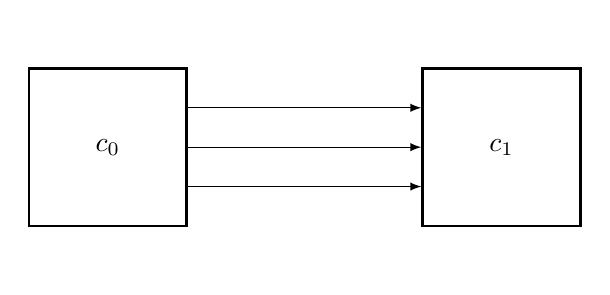
\begin{tikzpicture}
                                [
                                    square/.style = {draw, shape=rectangle, minimum height=2cm, minimum width=2cm, node distance=2cm, line width=1pt},
                                    empty/.style = {draw, shape=rectangle, minimum height=2cm, minimum width=2cm, node distance=2cm, line width=1pt, draw=white},
                                ]

                                \node[empty] (0a) at (0,0.5)     {};
                                \node[empty] (0b) at (0,-0.5)     {};
                                \node[square] (0c) at (0,0)     {$c_0$};

                                \node[empty] (1a) at (5cm,0.5)   {};
                                \node[empty] (1b) at (5cm,-0.5)   {};
                                \node[square] (1c) at (5cm,0)   {$c_1$};
                                
                                \draw [-latex] (0a.east) -- (1a.west);
                                \draw [-latex] (0b.east) -- (1b.west);
                                \draw [-latex] (0c.east) -- (1c.west);

                            \end{tikzpicture}
                        }
                    \end{figure}
